% Beamer slide template prepared by Tom Clark <tom.clark@op.ac.nz>
% Otago Polytechnic
% Dec 2012

\documentclass[10pt]{beamer}
\usetheme{Dunedin}
\usepackage{graphicx}
\usepackage{fancyvrb}

\newcommand\codeHighlight[1]{\textcolor[rgb]{1,0,0}{\textbf{#1}}}

\title{State Pattern}

\author[IN710]{Object Oriented System Design}
\institute[Otago Polytechnic]{
  Otago Polytechnic \\
  Dunedin, New Zealand \\
}
\date{}
\begin{document}

%----------- titlepage ----------------------------------------------%
\begin{frame}[plain]
  \titlepage
\end{frame}

\begin{frame}
	\frametitle{Delegation in design patterns}
        \begin{itemize}
		\item In OO, \emph{delegation} takes place when an object
	holds an instance of another object as a field and 
	delegates the execution of a task to it.
        \item This provide a way to modify the behaviour of an object
	at runtime.
        \item We saw one example of this with the \emph{Strategy} pattern.
	\end{itemize}

\end{frame}

\begin{frame}
	\frametitle{Problem}
	\begin{itemize}
		\item Suppose we are writing a game.  In the game, we have
			non-player characters that should respond whenever a 
			player gets close to them.
		\item The NPCs respond differently depending on what they
			are doing.  They may be
			\begin{itemize}
				\item guarding
				\item resting
				\item hiding
		                \item hunting
				\item moving
			\end{itemize}
		\item These things are \emph{states}.  We could say that
			an NPC is is a ``guarding state''.
	\end{itemize}
\end{frame}
\begin{frame}
	\frametitle{Basic implementation}

	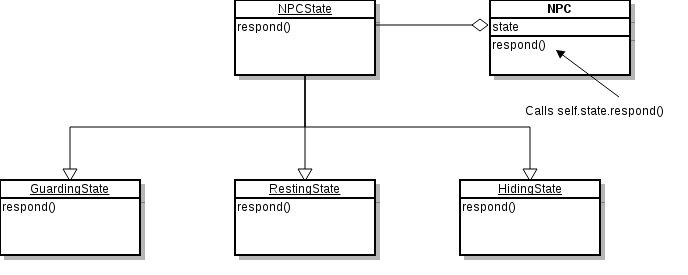
\includegraphics[width=100mm]{state-pattern.png}
\end{frame}
\begin{frame}
	\frametitle{So far, this looks like a strategy}

	They are related, but
	\begin{itemize}
		\item A state object can contain a lot
			of state related data.
		\item A state can implement many state-based
			behaviours.
		\item A state can control how the containing object
			transitions to other states.
	\end{itemize}
\end{frame}

\begin{frame}
	\frametitle{Exercises}

	\begin{enumerate}
		\item Write a \texttt{Light} class that uses two 
			state objects, \texttt{On} and \texttt{Off} to
			represent its states. The light should have a
			\texttt{switch()} method that delegates its
			implementation to the states.
		\item Write a \texttt{VendingMachine} class.  This class
			moves between a number of states, including 
			waiting, money-received, vending, and 
			making-change/refunding.  Implement a set
			of appropriate state classes.
	\end{enumerate}
\end{frame}

\end{document}
